\section{Theory}
This experiment explores the use of the Michelson interferometer to
determine the wavelength of visible light and perform other precision
measurements.

The basic principle of all interferometry measurements is that 
if two coherent light beams originate from a common source and 
travel different paths to a common end point, interference will 
occur at the end point. The nature of the interference is determined 
by the difference in the optical path lengths. A schematic diagram 
of a Michelson interferometer is shown in Figure~\ref{schematic} below.


\begin{figure}[htbp]
\begin{center}
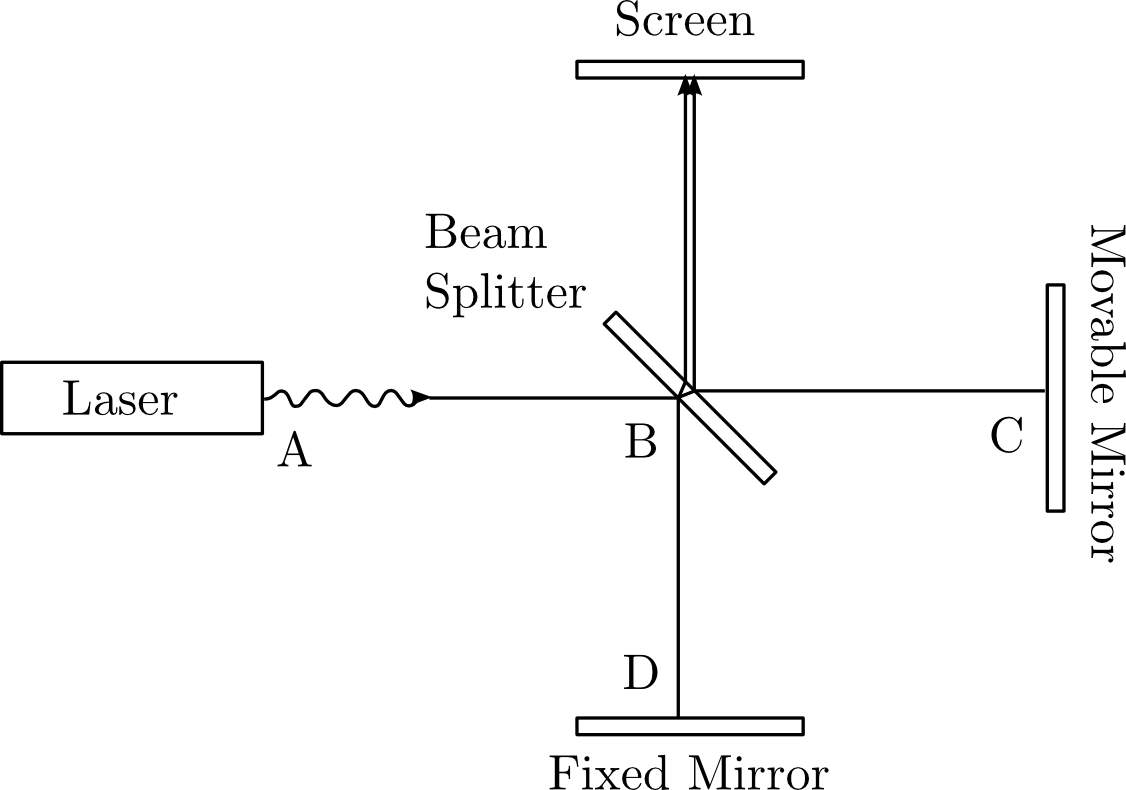
\includegraphics[width=0.6\textwidth]{../images/inter.png}
\caption{Michelson Interferometer }
\label{schematic}
\end{center}
\end{figure}


A monochromatic light beam enters the interferometer along line $AB$. At
$B$ the beam encounters a half-silvered mirror which functions as a beam
splitter. Part of the beam continues along the same direction, reflects
from the movable mirror at $C$ and returns to $B$. The remainder of the beam
reflects from the beam splitter, strikes the fixed mirror at $D$ and
returns to the beam splitter at $B$. The two beams recombine at $B$ and
travel together to the screen. 

During the time when the beams are split, they travel different 
paths. One path is of length equal to twice the distance from 
$B$ to $C$, denoted $\langle BC\rangle$. The other path length is twice 
the distance from $B$ to $D$, denoted $\langle BD\rangle$. The difference 
between these path lengths determines the nature of the interference 
seen at a particular point on the screen. If we let the difference in path lengths be $PD$, we have

\begin{equation}
PD = 2\langle BC\rangle - 2\langle BD\rangle 
\label{eq:pathlength}
\end{equation}

then the condition for constructive interference is 

\begin{equation}
 PD = m\lambda
\label{eq:constructive}
\end{equation}
and the condition for destructive interference is

\begin{equation}
PD = (m+1/2)\lambda
\label{eq:destructive}
\end{equation}

 In Eqs.~\ref{eq:constructive}~\&~\ref{eq:destructive}, $\lambda$ is the light wavelength and $m$ is 
an integer. In general the interference pattern on the screen 
will consist of alternating bright and dark regions (usually 
fine curved lines) called ``fringes''.

Turning the micrometer dial on the interferometer displaces the 
moveable mirror, changing the distance $\langle BC \rangle$, while $\langle BD\rangle $
remains fixed. Thus, the path length difference $PD$ between the 
two beams can be varied in a controlled manner. If the distance 
$\langle BC\rangle$ changes from an initial value of $\langle BC\rangle_{1}$ 
to a final value $\langle BC\rangle_{2}$ , then, using Eq.~\ref{eq:pathlength}, the change 
in the path length difference PD is given by:

\begin{equation}
 PD_2 - PD_{1} = 2\langle BC\rangle_{2} - 2\langle BD\rangle - (2\langle BC\rangle_{1} - 
2\langle BD\rangle).
\label{eq:deltapathlength}
\end{equation}


Hence,

\begin{equation}
PD_{2} - PD_{1} = 2(\langle BC\rangle_{2}  - \langle BC\rangle_{1}) = 2(d_{2} - 
d_{1})
\end{equation}

where $d_{1}$ is the initial micrometer reading and $d_{2}$ is the  final micrometer reading.

Each time PD changes by one wavelength $\lambda$, the integer $m$ changes
by one unit (see Eqs.~\ref{eq:constructive}~\&~\ref{eq:destructive}), and the observed pattern of interference
fringes shifts by one fringe. As the micrometer reading changes from
$d_{1}$ to $d_{2}$, $m$ will change from $m_{1}$ to $m_{2}$. Combining
Eqs.~\ref{eq:constructive} and ~\ref{eq:deltapathlength}, we can express

\begin{align}
 \Delta m &= m_2 - m_1 \nonumber \\
 &= \frac{PD_{2}}{\lambda} - \frac{PD_{1}}{\lambda} \nonumber \\
 &= \frac{2(d_{2} - d_{1})} {\lambda} \nonumber
\end{align}
so
\begin{equation}
\boxed{\Delta m = \frac{2(d_{2} - d_{1})} {\lambda}}
\label{eq:delta-m}
\end{equation}
where $\Delta m$ is the number of fringes shifted past a fixed point as the micrometer 
dial reading changes from $d_{1}$ to $d_{2}$.

On this apparatus, the micrometer dial is designed so that one 
complete revolution of the micrometer dial corresponds to a change 
$d_{2} - d_{1} = 25 \mu$m.


NOTE: 1 $\mu$m $= 10^{-6}$ m.

%\subsection{Calibration of Michelson Interferometer}
%
%For precise work one can calibrate the micrometer dial by counting 
%the fringes shifted due to a given micrometer movement, if the 
%wavelength of the light source is known. Assume that \ensuremath{\Delta}m 
%fringes are shifted by a change d$_{2}^\prime$ - d$_{1}^\prime$ of the micrometer 
%dial. Using Eq.~\ref{eq:delta-m} we can calculate the change d$_{2}$ - d$_{1}$ expected 
%for perfect calibration. We then define the correction factor 
%$F$ as: 

%\begin{equation}
%\boxed{ F = {(d_2- d_1) \over (d_2^\prime - d_1^\prime)} }
%\label{eq:calibration}
%\end{equation}

%Once $F$ is determined, it may be used to correct other measurements. 
%One simply multiplies any micrometer dial reading change $d_2^\prime - 
%d_1^\prime $ by $F$ to obtain the corrected value $d_2 - d_1$.


\subsection{Index of refraction of a glass slide}

It is difficult to measure the index of refraction of a thin 
slab of transparent material by observing refraction, because 
a beam refracted within the material will return to its original 
direction after exiting the slab. Although the beam is shifted 
slightly parallel to itself, this effect is not normally easily 
measurable. An attractive solution to this problem is to measure 
the fringe shift occurring when the slab is rotated in the path 
of one of the interferometer beams--while the other beam is unchanged. 
This rotation causes the light beam to traverse a thicker portion 
of the material, as the slab is turned away from being perpendicular 
to the light beam. Since the light wavelength is shorter in the 
slab than in air (why?), the beam passing through the slab will 
contain increasingly more wavelengths as the angle from the perpendicular 
orientation increases. For each additional wavelength contained 
in the slab (compared to an equal thickness of air), the interference 
fringe pattern will shift by one fringe.

Thus, there is a relationship between the following quantities:

\begin{description}

\item[$n$]  the index of refraction of the slab
\item[$t$]  the thickness of the slab
\item[$\theta$]  the angle through which the slab is rotated, relative to an  initial position in which the slab is perpendicular to the  incident light beam
\item[$\Delta m$]  the number of fringes passing a fixed point when the slab 
is  rotated by angle \ensuremath{\theta} from its initial position.

\end{description}


To a good approximation, it can be shown that this relationship 
is:

\begin{equation}
\boxed{ n = { t - \lambda ( \Delta m/2) \over t - \left[ \lambda ( \Delta m/2)/(1-\cos\theta) \right] }
\label{eq:glassslide}}
\end{equation}


\subsection{Index of refraction of a gas}

If one of the interferometer beams travels through a sealed chamber, 
that beam will travel more rapidly inside the chamber than it 
would outside the chamber if the pressure of the air inside the 
chamber is less than normal atmospheric pressure (i.e. closer 
to being a vacuum).

This means that the index of refraction n of air actually depends 
on the air pressure $P$, and we shall denote this index of refraction 
as $n_P$ . Since the light frequency is unaffected by changes in 
the medium, the wavelength of the light being used depends on 
the index of refraction in the same way as the velocity of light, 
i.e.


\begin{equation}
\lambda_P = {\lambda \over n_P}
\label{eq:lambdaP}
\end{equation}

where $\lambda$ is the wavelength of the light in a vacuum, 
and $\lambda_P$ is the wavelength in air at pressure $P$.

In this experiment, we form the usual interference pattern with 
the two interferometer beams, but now with one of the beams traveling 
through the air chamber. At the initial atmospheric pressure, 
the number of wavelengths of light contained in the air chamber 
is equal to $2t/\lambda_{\rm atm}$, where t is the thickness of 
the air layer in the chamber measured along the light path. (Why 
does the factor of 2 occur?) As the pressure inside the chamber 
decreases, $n_P$ decreases, $\lambda_P$ increases, and fewer 
wavelengths are contained inside the chamber. The change in the 
number of wavelengths in the chamber as the pressure is varied 
will equal the number $\Delta m$ of fringes that move past a 
fixed point in the interference pattern. 

In the experiment, we begin with the air pressure in the chamber 
equal to atmospheric pressure, so that the index of refraction 
initially is $n_{\rm atm}$. The pressure is then decreased to a value 
$P$. The number of wavelengths inside the chamber decreases to 
$2t/\lambda_P$, and it follows that


\begin{align}
\Delta m &= 2t/\lambda_{\rm atm} - 2t/\lambda_P \nonumber \\
 &= (2t/\lambda ) ( n_{\rm atm} - n_P ) 
\label{eq:delta-m-P}
\end{align}

where $\Delta m$ is the number of fringes passing a fixed point while the 
gas pressure in the chamber varies from atmospheric pressure to a pressure $P$,
and where the second equality was obtained using Eq.~\ref{eq:lambdaP}.

At a final gas pressure of zero in the chamber (a perfect vacuum), 
$n_P = 1$, and Eq.~\ref{eq:delta-m-P} becomes
\begin{equation}
\boxed{ (\Delta m)_{P=0} = \frac{2t}{\lambda}(n_{\rm atm} - 1)}
\label{eq:delta-m-P0}
\end{equation}

Although $(\Delta m)_{P=0}$ is not directly measurable (because 
we cannot obtain a perfect vacuum in the chamber), it can be 
determined from the other $\Delta m$ measurements by graphical 
extrapolation. Knowing it, we can then use Eq.~\ref{eq:delta-m-P0} to find $n_{atm}$, 
the index of refraction of air at atmospheric pressure.



\section{Preliminary Question}

\begin{enumerate}
\item A monochromatic light source is used in a Michelson interferometer. 
The micrometer dial controlling the moveable mirror is rotated 
until 100 interference fringes pass a fixed point. The difference 
between the final and initial micrometer readings is 32.0 microns, 
This is the displacement of the moveable mirror. 

Use the given information to determine the wavelength of the 
light. 

% HINT: Use Equation~\ref{eq:delta-m}.
\end{enumerate}


\section{Equipment}
PASCO Michelson interferometer, laser, lens, screen, 
mounted glass slide, micrometer, gas cell


 \section{Procedure}

Caution: IN THOSE PORTIONS OF THE EXPERIMENT USING A LASER LIGHT 
SOURCE, BE CAREFUL NOT TO LOOK DIRECTLY INTO THE BEAM OR TO LET 
A DIRECT REFLECTION OF THE BEAM ENTER YOUR EYE.


\begin{enumerate}

\item Adjustment of Michelson interferometer

\begin{enumerate}
\item Use a He-Ne laser beam with the interferometer set up as 
in Fig.~\ref{schematic}. By adjusting the orientation of the fixed mirror, 
align the two recombined interferometer beams so that they are 
superimposed on the screen. 
\item Insert a lens between the laser and the beam splitter to 
broaden the laser beam. Observe the interference fringes projected 
on a screen.
\item Carefully adjust the lens and the orientation of the fixed 
mirror to obtain an interference pattern of concentric rings 
(resembling a target with a ``bulls-eye''). Explain 
why a ring pattern is formed. HINT: What is the shape of the 
laser light wave fronts when the lens is present?
\end{enumerate}



%\item Calibration of Michelson interferometer
%
%\begin{enumerate}
%\item Set the micrometer dial to a low (but not zero) reading. 
%Record this reading. Then advance the micrometer dial until 30 
%fringes (i.e. bright rings) have passed a fixed point on the 
%screen, and record the micrometer dial reading. Repeat this process 
%three more times using different parts of the micrometer dial 
%scale, but not too close to the ends of the scale.

%Note: The micrometer dial is designed so that one complete 
%revolution of the micrometer dial corresponds to a change $d_2 - 
%d_1 = 25$ microns. Note: $1 {\rm micron } = 1 \mu {\rm m} = 10^{-6} {\rm m}$.


 
%\item Compute the average value of the shift in mirror position 
%$d_2^\prime - d_1^\prime$ for the four trials in step a. Referring to the 
%theory section, find the correction factor $F$ (Note: He-Ne Laser 
%light wavelength in a vacuum $= \lambda = 632.8$ nm). Check 
%your results with the instructor. Your value of $F$ will be used 
%in analyzing results of some of the other interferometer measurements. 
%\end{enumerate}

\item \label{proc:lambda} Measuring the wavelength of a He-Ne laser

The wavelength of the laser can be determined by using the micrometer
dial to displace the movable mirror by a known amount and counting
the corresponding number of fringes that pass by on the screen.
Count a fairly large number of fringes, say roughly 30, and note the
micrometer reading before and after.  Repeat this measurement several
times using different parts of the micrometer dial to reduce errors from
nonlinearities in the mirror mechanism..

\item Qualitative observations

\begin{enumerate}
\item What happens to the interference pattern when an opaque sheet 
is placed in the path of one of the two beams produced by the 
interferometer before they recombine. Why?

\item What happens to the interference pattern when the table holding 
the interferometer is tapped or lightly jarred? Explain the sensitivity 
of the pattern to these perturbations.
\end{enumerate}

 \item Index of refraction of a glass slide

Note: the micrometer dial controlling the moveable mirror is 
not used in this part of the experiment. 

\begin{enumerate}
\item We use the laser light source and a glass slide as a sample.
The glass slide is mounted on a magnetic holder placed at the center of a
table which allows it to be rotated about a vertical axis.  The angle of
rotation can be read using the scale printed on the interferometer base.
The interferometer is designed so that slide is in the path of the laser
beam passing between the beam splitter and the moveable mirror of the
interferometer (path $BC$ in Fig.~\ref{schematic}).

\item Align the slide initially so that its plane is perpendicular 
to the laser beam passing through it. The fringe pattern itself 
can be used to determine this position - it is the point at which 
the fringes begin to reverse direction as the slide is slowly 
rotated (why?). 

SUGGESTION: To accomplish the alignment, set the rotating table 
so that its arm is accurately at zero on the angular scale. Then, 
without allowing the table to move, carefully rotate the mount 
holding the glass slide until you observe the reversal of the 
fringe motion. Position the slide at the turning point just before 
the reversal begins. 

\item Slowly rotate the table by moving its arm (without touching 
the slide), counting the number of fringes passing a fixed point. Continue until you 
reach 100 fringes, or until you reach the maximum calibrated 
angle (20 degrees) -- whichever comes first. Record the number 
of fringes counted and the angle $\theta$ through which the 
slide has been rotated ($\theta$ should be determined to the 
nearest tenth of a degree). 

Also, measure the thickness of the slide with a micrometer to 
three significant figures.
\end{enumerate}

\item Index of refraction of a gas

Note: the micrometer dial controlling the moveable mirror is 
not used in this experiment.

Mount the gas cell so that one of the interferometer beams passes 
through it, perpendicular to its side windows. Count the fringes 
passing a fixed point as the pressure in the chamber is slowly 
reduced from atmospheric to the minimum value obtainable. Record 
the {\em cumulative number of fringes passing} (starting from 
atmospheric pressure) for each increment of 10 cmHg of pressure 
decrease. 


Note that the pressure gauge is actually a vacuum gauge, and 
gives a reading of the {\em pressure decrease} $\Delta P = 
P_{\rm atm} - P$ in cmHg, where $P_{\rm atm}$ is atmospheric pressure and $P$ 
is the pressure in the chamber. $P_{\rm atm}$ is approximately equal 
to 76 cmHg, and can be determined more precisely from a barometer. 
Also, measure the thickness $t$ of the air space in the chamber 
along the light path.


\end{enumerate}

\section{Analysis}


(Note: For a He-Ne Laser light wavelength in a vacuum $ \lambda
= 632.8$ nm). 


\begin{enumerate}
\item Compute the wavelength of the laser light using the data you collected in procedure step~\ref{proc:lambda} using Eq.~\ref{eq:delta-m}

\item Compute, using Eq.~\ref{eq:glassslide}, the index of refraction of the glass 
slide studied in Procedure step 4. Compare to typical tabulated 
values of the index of refraction of glass. 

NOTE: Eq.~\ref{eq:glassslide} is complicated and care must be taken in the computation. 
Do not round off numerical data values or any intermediate numerical 
results. How many significant figures should your final result 
for $n$ have?

\item Plot the cumulative number of fringes $\Delta m$ passing 
as a function of the pressure decrease $\Delta P = P_{\rm atm} - 
P$ for your data taken with the gas cell. Draw the best straight 
line through your points (or use a computer curve fit). Extrapolate 
your graph to pressure $P = 0$ (i.e., to pressure decrease $\Delta P 
= P_{\rm atm}$), and determine $(\Delta m)_{P=0}$ from the extrapolated 
line. 

Then use Eq.~\ref{eq:delta-m-P0} to calculate the index of refraction of air 
at atmospheric pressure, $n_{\rm atm}$. Compare this result to a tabulated 
value. Suggestion: First compute $n_{atm} - 1$ using 
Eq.~\ref{eq:delta-m-P0} . Then you can easily write the result for $n_{\rm atm}$ itself. Note: 
The calculated $n_{\rm atm}$ will be slightly greater than 1, and {\em the 
final result must not be rounded off to 1.0 !}



\end{enumerate}

%\section{References}
%Serway and Jewett, {\underline {Physics for Scientists and 
%Engineers}}, 6$^{th}$ edition, pp. 1177-1181, 1194 

